\documentclass[a4paper]{article}
\usepackage[spanish]{babel}
\title{Trabajo Práctico 1}

\usepackage[utf8]{inputenc}
\usepackage{caratula}
\usepackage{graphicx}
\usepackage{color}
\usepackage{listings}
\usepackage{float}

\setlength{\leftmargin}{2cm}
\setlength{\rightmargin}{2cm}
\setlength{\oddsidemargin}{-1cm}
\setlength{\evensidemargin}{-1cm}
\setlength{\topmargin}{-1cm}
\setlength{\textwidth}{18cm}
\setlength{\textheight}{25cm}

\usepackage{fancyhdr}
\pagestyle{fancy}
\fancyhf{}
\fancyhead [LO,LE]{\scriptsize Trabajo Práctico N$^{\circ}$1}
\fancyhead [RO,RE]{\scriptsize Mancuso, Mataloni, Tolchinsky}
\fancyfoot[CE,CO]{\thepage}
\renewcommand{\footrulewidth}{0.4pt}

\usepackage[pdftex, bookmarks=true, colorlinks, citecolor=black, linkcolor=black]{hyperref}
\usepackage{multirow}

\begin{document}

\materia{Métodos Numéricos}
\submateria{Primer Cuatrimestre de 2012}
\titulo{Aproximación de Ceros o Raíces de una función. }
\subtitulo{ Aproximación Numérica,  Bisección, Newton-Raphson }
\grupo{Trabajo Práctico N$^{\circ}$1}
\integrante{Mancuso, Emiliano}{597/07}{emiliano.mancuso@gmail.com}
\integrante{Mataloni, Alejandro}{706/07}{amataloni@gmail.com}
\integrante{Tolchinsky, Lucas}{591/07}{lucas.tolchinsky@gmail.com}
\maketitle
\newpage

\addcontentsline{toc}{section}{Índice}
\tableofcontents

% Main project

\newpage
\section{Resumen TODO}
%El resumen, de no más de 200 palabras, debería explicar brevemente el trabajo realizado y las conclusiones de los autores de manera que pueda ser u ́til por s ́ı solo para dar una idea del contenido del trabajo. Las palabras clave, no m ́as de cuatro, deben ser t ́erminos t ́ecnicos que den una idea del contenido del trabajo para facilitar su bu ́squeda en una base de datos tem ́atica.
El trabajo implementa un programa que permite aproximar la raíz de una función por los métodos de \textbf{Bisección} y \textbf{Newton-Raphson}, utilizando para esto aritmética de punto flotante variando la precisión de la mantisa, hasta un máximo de 52 bits. En cuanto a la calidad de resultados ambos algoritmos nos proporcionan la misma precisión, sólo que \textbf{Newton} lo hace con un orden de convergencia cuadrático (contra el lineal de \textbf{Bisección}). Sin embargo, éste necesita una \textit{semilla} inicial cercana a la raíz buscada para asegurar la convergencia, por lo que decidimos implementar una combinación de ambos, aplicando primero \textbf{Bisección} para encontrar un punto inicial cercano, y luego aplicar \textbf{Newton} desde la semilla encontrada.  


\section{Introducción Teórica}
%Contendr ́a una breve explicaci ́on de la base te ́orica que fundamenta los m ́etodos involu- crados en el trabajo, junto con los m ́etodos mismos. No deben incluirse demostraciones de propiedades ni teoremas, ejemplos innecesarios, ni definiciones elementales (como por ejemplo la de matriz sim ́etrica). En vez de definiciones b ́asicas es conveniente citar ejemplos de bibliograf ́ıa adecuada. Una cita vale m ́as que mil palabras.
Sea $f(x)$ una función, un problema interesante a resolver es el de encontrar todos los $x$ pertenecientes al dominio de $f$ tal que $\mathbf{f(x) = 0}$. Para resolver este problema se conocen varias técnicas que utilizaremos en este trabajo. Supongamos que el dominio de $f$ son los números reales. Dado que vamos a resolver el problema con una computadora nos encontramos frente al primer inconveniente. Las maquinas tienen una cantidad acotada de bits para representar los números. Es por esto que no todos los números pueden ser representados, por ejemplo $\sqrt(3)$ no puede ser representado ya que es irracional y tiene infinitas cifras decimales. Es por esta razon que los algoritmos no pueden dar una solución exacta a este problema, aunque si lo bastante cercana a la misma para que sea aceptable en la mayor parte de las situaciones.  
  
\subsection{Bisección}
También conocido como método de \textbf{Búsqueda binaria}, se basa en el teorema del valor intermedio. 
Requiere dividir varias veces a la mitad los subintervalos de [a,b] y, en cada paso, localizar la mitad que 
contenga a \textbf{p}, tal que $\mathbf{f(p) = 0}$.
Si bien tiene una importante propiedad, que asegura la convergencia en una solución, 
esta convergencia puede ser muy lenta. 
Por eso, a menudo se utiliza para iniciar otros métodos mas eficientes, como por ejemplo \textbf{Newton-Raphson}.

\subsection{Newton-Raphson}
El \textbf{método de Newton-Raphson} es una de las técnicas más eficientes para calcular ceros de función,
dado que nos provee convergencia cuadrática. El método precisa de un $\mathbf{x_0}$ cercano 
al \textbf{p} tal que $\mathbf{f(p) = 0}$ y la ecuación del mismo se inspira en el desarrollo de
Taylor de grado dos alrededor de $\mathbf{x_0}$:

$$f(x) = f(x_0) + (x - x_0)f'(x_0) + \frac{(x - x_0)^2}{2}f''(x_0)$$
Evaluando en \textbf{p}:
$$0 = f(x_0) + (p - x_0)f'(x_0) + \frac{(p - x_0)^2}{2}f''(x_0)$$
Como  $|p - x_0|$ es muy chico $(p - x_0)^2 \approx 0$, luego:  
$$0 \approx f(x_0) + (p - x_0)f'(x_0)$$
$$p \approx x_0 - \frac{f(x_0)}{f'(x_0)}$$

De esta manera, podemos generar la serie $x_{n + 1} = x_n - \frac{f(x_n)}{f'(x_n)}$ que, arrancando de un $x_0$ adecuado, converge a \textbf{p}.

% Discutir si anexamos la demostración de este punto.

\section{Desarrollo TO BE CONTINUED}
%Deben explicarse los m ́etodos num ́ericos que utilizaron y su aplicaci ́on al problema concreto involucrado en el trabajo pr ́actico. Se deben mencionar los pasos que si- guieron para implementar los algoritmos, las dificultades que fueron encontrando y la descripci ́on de c ́omo las fueron resolviendo. Explicar tambi ́en c ́omo fueron planteadas y realizadas las mediciones experimentales. Los ensayos fallidos, hip ́otesis y conjeturas equivocadas, experimentos y m ́etodos malogrados deben figurar en esta secci ́on, con una breve explicaci ́on de los motivos de estas fallas (en caso de ser conocidas).

Para resolver lo planteado por el trabajo práctico decidimos dividir el problema en tres etapas:
\begin{enumerate}
\item Primer impacto
\item Altura máxima del rebote
\item Segundo impacto
\end{enumerate}
Para cada una de ellas, aplicamos los algoritmos de Bisección y Newton. En 1 y 3, sobre las ecuacines de la posición y en 2, sobre las ecuaciones de velocidad.
El código está escrito en el lenguaje C y en cuanto a la implementación nos topamos con varias dificultades que desarrollaremos a continuación.
\begin{description}
\item \textbf{Parámetros}\\
Dado que las instancias de este problema son muy variadas en cuanto a la cantidad de variables a tener en cuenta, como posición y velocidad inical, cantidad máxima de iteraciones de los algoritmos, tolerancia del resultado, etc, la primer dificultad que encontramos fue poder generar un binario al que fuera cómodo pasarle los diferentes valores. Para eso utilizamos la biblioteca \textit{getopt} de C que parsea los parámetros del CLI.
\item \textbf{Ecuaciones}\\
Este trabajo práctico nos propone dos modelos del problema de caída libre y rebote: uno con rozamiento y uno sin rozamiento. Para esto nos provee de dos pares de ecuaciones de posición y velocidad, contemplando ambas situaciones, lo cual en un principio nos llevó a escribir dos versiones de cada algoritmo, con la única diferencia de que en una se utilizaban las ecuaciones sin rozamiento y en la otra, con.
El problema con esto es que hace un código más complejo, más largo y propenso a errores. Finalmente este punto fue resuelto implementando una única vez los algoritmos de Bisección y Newton, haciéndolos recibir punteros a función, según el caso correspondiente.
\item \textbf{Presición y representación numérica}\\
Con motivo de minimizar el error de representación en los números, la cátedra nos facilitó una clase de C++ que nos permite representar los números de punto flotante con una cantidad determinada de bits en la mantisa, sin importar las operaciones que se realicen entre ellos. EXPLICAR ACA EL PROBLEMA DEL PRINTF Y LA CANTIDAD DE DECIMALES.

\end{description} 

\section{Resultados}

\begin{figure}[H]
  \centering
  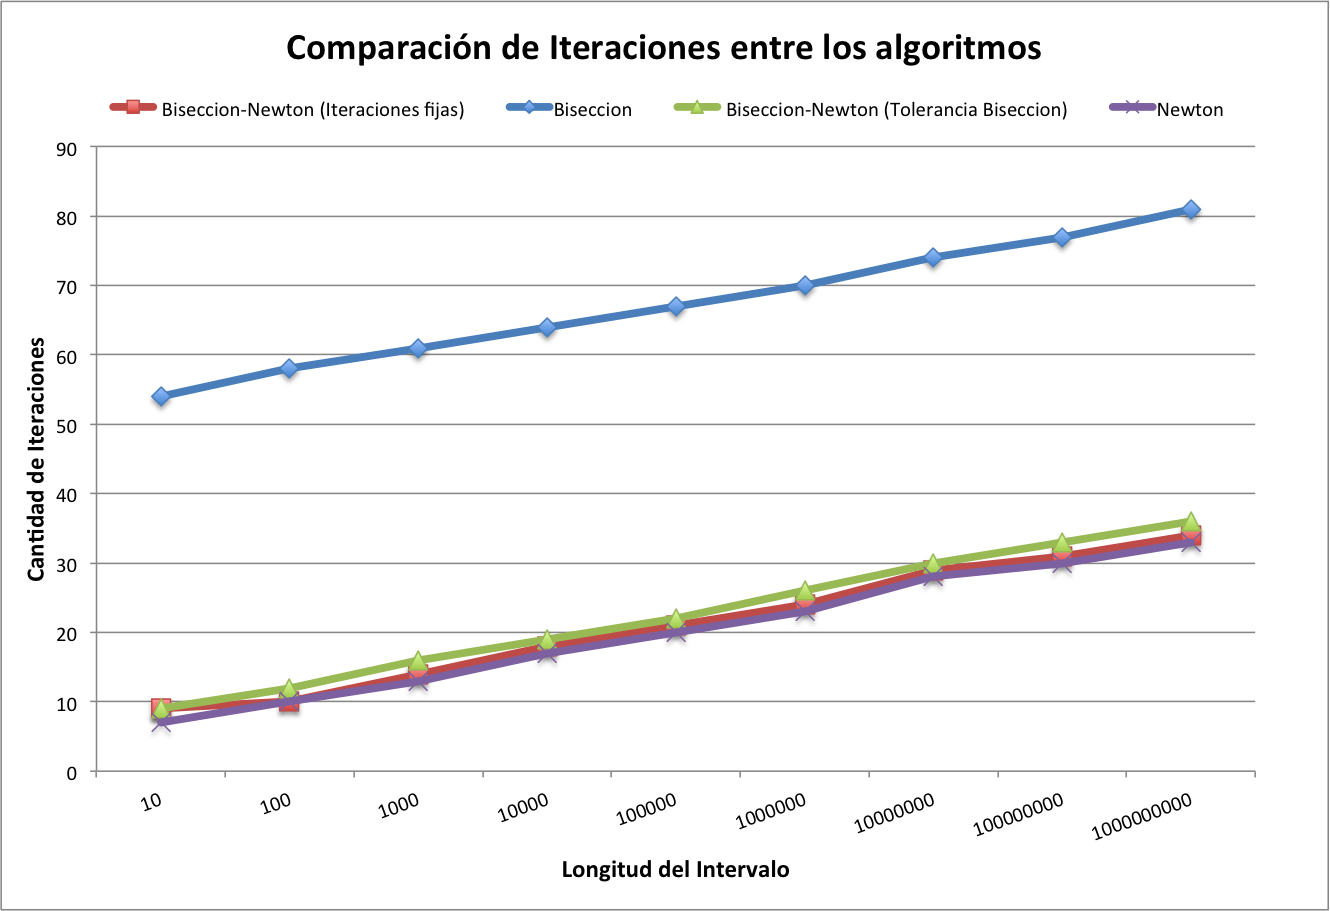
\includegraphics[scale=0.80]{graficos/1-Biseccion_vs_BiseccionNewton.png}
  \caption{Cantidad de Iteraciones. Bisección vs Newton (con aproximación de Bisección) }
\end{figure}

\begin{figure}[H]
  \centering
  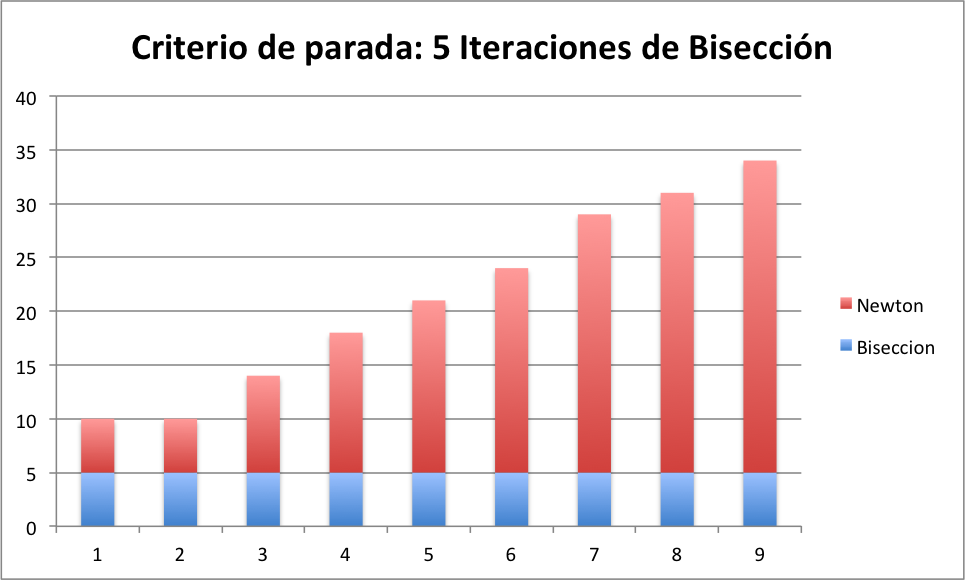
\includegraphics[scale=0.80]{graficos/2-BiseccionXIteraciones.png}
  \caption{Aproximación con Bisección limitada a 5 iteraciones. }
\end{figure}

\begin{figure}[H]
  \centering
  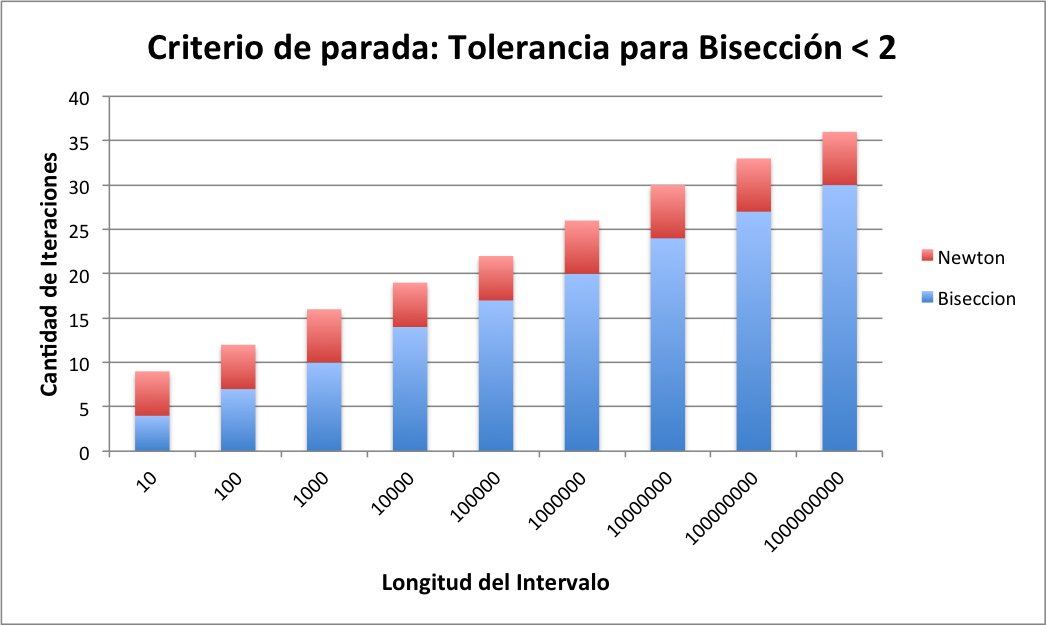
\includegraphics[scale=0.80]{graficos/3-BiseccionXTolerancia.png}
  \caption{Aproximación con Bisección limitada a una tolerancia de 2. }
\end{figure}

\begin{figure}[H]
  \centering
  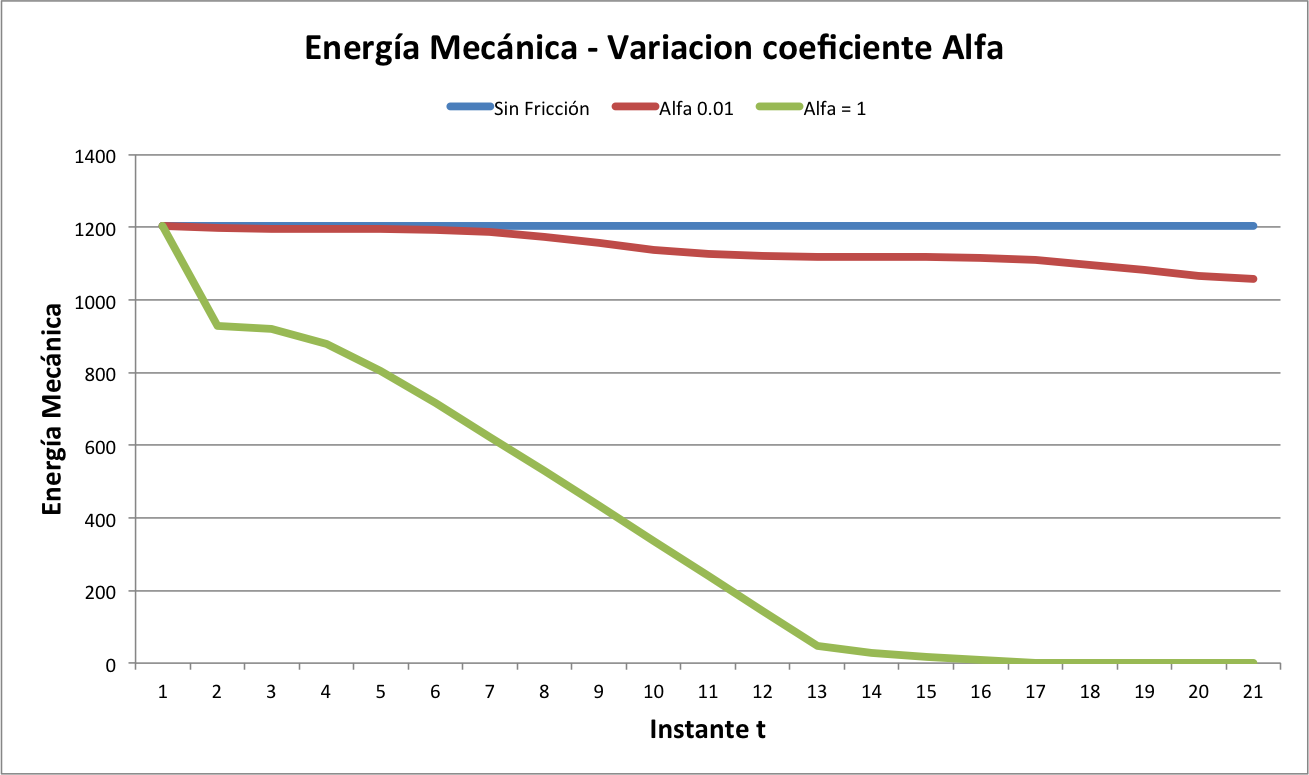
\includegraphics[scale=0.75]{graficos/4-energiaMecanica-alpha.png}
  \caption{Comparación diferencia de energía mecánica. Variando \alpha }
\end{figure}

\begin{figure}[H]
  \centering
  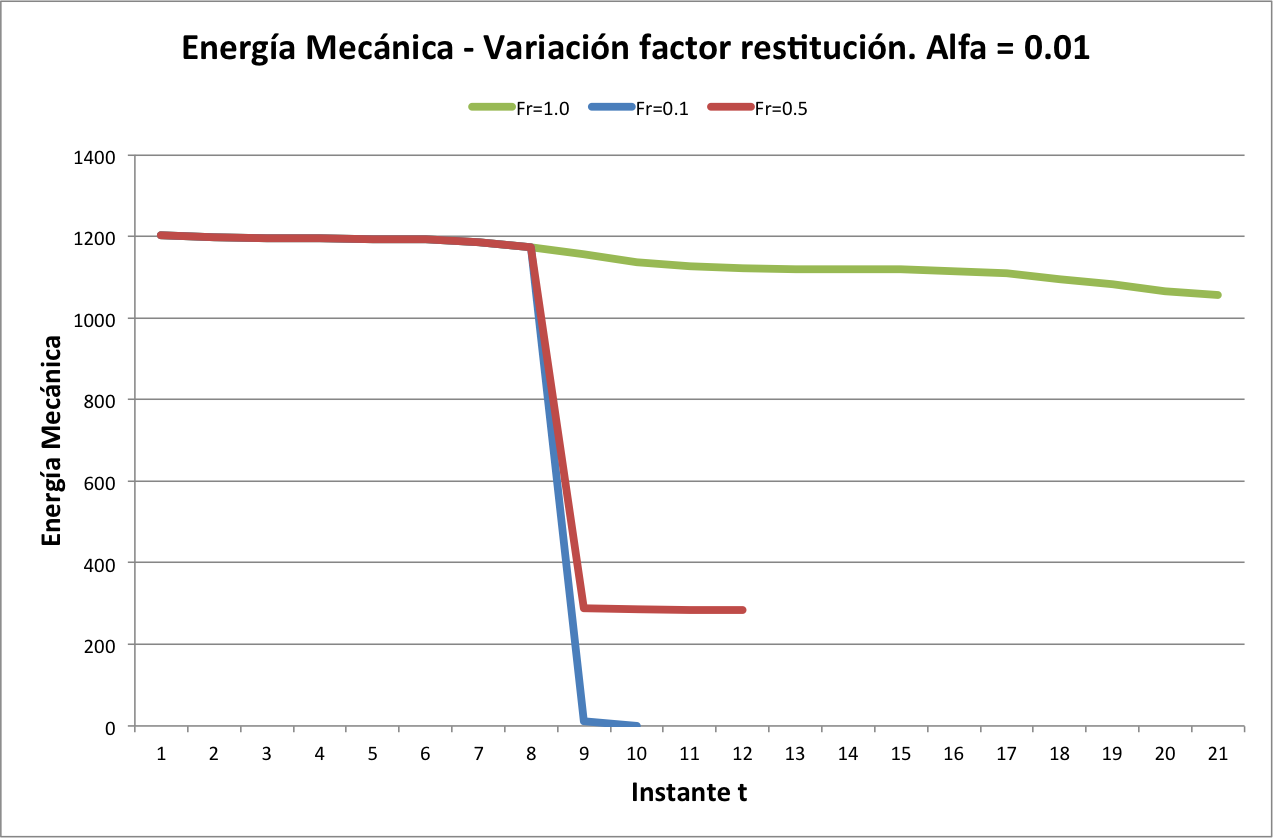
\includegraphics[scale=0.75]{graficos/5-energiaMecanica-fr.png}
  \caption{Comparación diferencia de energía mecánica. Variando \textit{Fr} }
\end{figure}


%Deben incluir los resultados de los experimentos, utilizando el formato m ́as adecuado para su presentaci ́on. Deber ́an especificar claramente a qu ́e experiencia corresponde cada resultado. No se incluir ́an aqu ́ı corridas de m ́aquina. Algo fundamental en su aprendizaje en la materia es la presentaci ́on de resultados de forma clara y concisa para el lector.

\section{Discusión TODO}
Sabiendo que el método de \textbf{Newton-Raphson} converge de forma cuadrática, decidímos comparar la cantidad de iteraciones que requiere cada algoritmo para mostrar de forma gráfica la eficiencia de los mismos. \\

Para esto, nos centramos en resolver el problema con parámetros fijos de solución exacta.
Los gráficos representan los resultados con los siguientes parámetros, 
\begin{itemize}
  \item{G = 9.81}
  \item{Velocidad Inicial = 29.43 (3G)} 
  \item{Altura Inicial = 78.48 (8G)} 
  \item{Tolerancia = $10^{-14}$} 
  \item{Máx. Iteraciones = $10^5$}
\end{itemize}

Bajo estas condiciones, es fácil probar que la solución es exactamente 8, basta con resolver la siguiente ecuación cuadrática:

\begin{displaymath}
  \frac{-3G \pm \sqrt{9G^2 + 4*\frac{G}{2}*8G}}{-2\frac{G}{2}}
\end{displaymath}

Ahora, con este problema bien definido, variamos la longitud del intervalo donde comienza \textbf{bisección} y graficamos la cantidad de iteraciones que necesita cada algoritmo (\textit{Figura 1}).
En primer lugar, encontramos una gran diferencia entre la cantidad de iteraciones necesarias por parte de \textbf{Bisección puro} y \textbf{Bisección + Newton}. Sin embargo, necesitabamos un criterio de aproximacion por Bisección para la semilla de Newton, y decidimos probar las 2 alternativas. 


%Agregado por Ale. Corregir y formatear

Otra prueba que realizamos fue para fijar el parámetro de parada para bisección cuando lo utilizabamos para darle una "semilla" a Newton. Teníamos dos alternativas: iterar una cantidad fija de veces, o acercarnos al valor a una distancia d.
En el gráfico podemos observar que no variaba mucho la cantidad final de iteraciones del algoritmo total para encontrar la raiz, por lo que dado que para este problema en particular Newton se comporta "bien" para una semilla aleatoria, decidimos utilizar una cantidad fija de iteraciones.
Si en algun otro problema fuera necesario tener una semilla buena, en ese caso se optaria por el otro criterio de parada.
 
 
%Se incluira aquı un analisis de los resultados obtenidos en la seccion anterior (se analizara su validez, coherencia, etc.). Deben analizarse como mınimo los ıtems pedidos en el enunciado. No es aceptable decir que “los resultados fueron los esperados”, sin hacer clara referencia a la teor ́ıa a la cual se ajustan. Adem ́as, se deben mencionar los resul- tados interesantes y los casos “patol ́ogicos” encontrados.

\section{Conclusiones TODO}
%Esta secci ́on debe contener las conclusiones generales del trabajo. Se deben mencionar las relaciones de la discusi ́on sobre las que se tiene certeza, junto con comentarios y observaciones generales aplicables a todo el proceso. Mencionar tambi ́en posibles extensiones a los m ́etodos, experimentos que hayan quedado pendientes, etc.

\newpage

\section{Apéndices}
\subsection{A - Enunciado}

En este trabajo práctico se deberá hacer un programa que, dadas las características del cuerpo (masa y coeficiente de rozamiento) y las condiciones iniciales (altura y velocidad de lanzamiento) calcule el momento en que se produce el primer impacto contra el suelo y la velocidad en ese instante. Asumir que la aceleración de la gravedad es $g = 9.81$ m/s$^2$.

Utilizando este programa:
\begin{enumerate}
  \item Analizar el efecto de la precisión numérica utilizada y las tolerancias adoptadas en la solución obtenida al calcular el primer impacto.
  
  \item Considerar que luego del primer impacto el cuerpo ``rebota'' en el suelo de manera no elástica, calcular la altura máxima del objeto luego del primer rebote y el momento del segundo impacto.

  \item ¿Cómo varía la energía mecánica ($E = g y +\dot{y}^2/2$) del cuerpo entre el lanzamiento y el segundo rebote? Estudiar el efecto de $\alpha$ (donde $\alpha = 0$ implica considerar el caso sin rozamiento), $f_r$ y la precisión numérica en esta variación.
\end{enumerate}

\subsection{B - Códigos Fuente}

\subsubsection{Stopping criteria}
\begin{verbatim}
bool stopping_criteria(double a, double b, double tolerance) {
  return fabs(a - b) < tolerance;
}
\end{verbatim}

\subsubsection{Bisección}
\begin{verbatim}
Result zero_bisection(Params *p, double (*fn)(Params *, double)) {
  int  iteracion = p->max_iterations;
  double a = p->a, b = p->b, m;
  Result res;

  while( --iteracion > 0 && !stopping_criteria(a,b, p->tolerance)) {
     res.zero = (b+a)/2;
    ( fn(p,a) * fn(p, res.zero) > 0 )? a = res.zero : b =  res.zero;
  }

  return res;
}
\end{verbatim}


\subsubsection{Newton-Raphson}
\begin{verbatim}
Result zero_newton(Params* p, double (*fn)(Params *, double), double (*deriv) (Params *, double)){
  double current = p->x, previous = 0.0;
  Result res;

  for(int i = p->max_iterations; i > 0 && !stopping_criteria(previous, current, p->tolerance); i--){
    previous = current;
    current = previous - (fn(p, previous)/deriv(p, previous));
  }

  res.speed = deriv(p,current);
  res.zero  = current;

  return res;
}
\end{verbatim}

\subsection{C - Cómo compilar y usar el TP}
El directorio del TP contiene un Makefile, con lo cual para compilarlo basta sólamente con ejecutar \textbf{make}. Los binarios generados son: 

\begin{itemize}
  \item \textbf{tp} Calcula primer impacto, altura máxima y segundo impacto.
  \item \textbf{mechanical\_energy} Para ver la variación de la energía mecánica. Utiliza metodos de bisección.
\end{itemize}

Y reciben los siguientes parámetros:

\begin{description}
\item[-M] es el método a ejecutar y se mapean del siguiente modo:
\begin{itemize}
  \item 0 para Bisección
  \item 1 para Bisección con fricción
  \item 2 para Newton
  \item 3 para Newton con fricción
  \item 4 para Bisección + Newton
  \item 5 para Bisección + Newton con fricción
\end{itemize}
\item[-h] posición inicial.
\item[-v] velocidad inicial.
\item[-t] tolerancia para Bisección.
\item[-m] masa de la pelota.
\item[-c] coeficiente de rozamiento.
\item[-f] factor de restitución.
\item[-i] cantidad máxima de iteraciones.
\item[-a] borde inicial del intervalo.
\item[-b] borde final del intervalo.
\item[-x] valor inicial para Newton.
\item[-z] tolerancia para Newton.
\end{description}

\newpage

\section{Referencias TODO}
%Es importante incluir referencias a libros, art ́ıculos y p ́aginas de Internet consultados durante el desarrollo del trabajo, haciendo referencia a estos materiales a lo largo del informe. Se deben citar tambi ́en las comunicaciones personales con otros grupos.

\end{document}
